\documentclass[10pt,a4paper,epsf,apalike]{article}

% Essential + Custom style packages
\usepackage[margin=1in]{geometry} % margins suitable for one page
\usepackage{graphicx} % include figures
\usepackage{amsmath,amsfonts,amssymb} % math symbols and fonts
\usepackage{dcolumn} % align table columns on decimal point
\usepackage{xcolor}
\definecolor{tabblue}{HTML}{1F77B4} % used by hyperref below
\usepackage[breaklinks=true,hidelinks,colorlinks=true,linkcolor=tabblue,citecolor=tabblue,urlcolor=tabblue]{hyperref}
\usepackage{enumitem} % control over lists
\usepackage{xurl} % allow long URLs to break across lines

% Custom colors and formatting
\usepackage{color}

% Header and footer settings
\usepackage{fancyhdr}
\pagestyle{fancy}
\fancyhf{}
\renewcommand{\headrulewidth}{0pt}
\lhead{\footnotesize Introduction to Data Analytics}
\chead{\footnotesize Airport Disruption Forecasting}
\rhead{\footnotesize \today}
\cfoot{}

% Line and paragraph spacing
\setlength{\parindent}{0pt}
\linespread{1.5}
\setlength{\parskip}{0.5em} % space between paragraphs
\hfuzz 1pt
\vfuzz 1pt

\newcommand{\repo}{https://github.com/sidnov6/airport-disruption-germany}

\begin{document}

%% Title and Highlight
\begin{center}
{\large\bfseries Airport disruption in Germany}\\[0.5em]
{\small Author 1, Author 2, and Author 3}\\[1em]
{\small Using only public EUROCONTROL and DWD data for 12 German airports, a LightGBM model ranked disrupted airport-days in 2024--2025 with average precision 0.39, against 0.24 for the previous 28-day disruption rate and a base rate of 0.06.}
\end{center}

%% Figure 1A (the other panels are linked below the Results)
\begin{center}
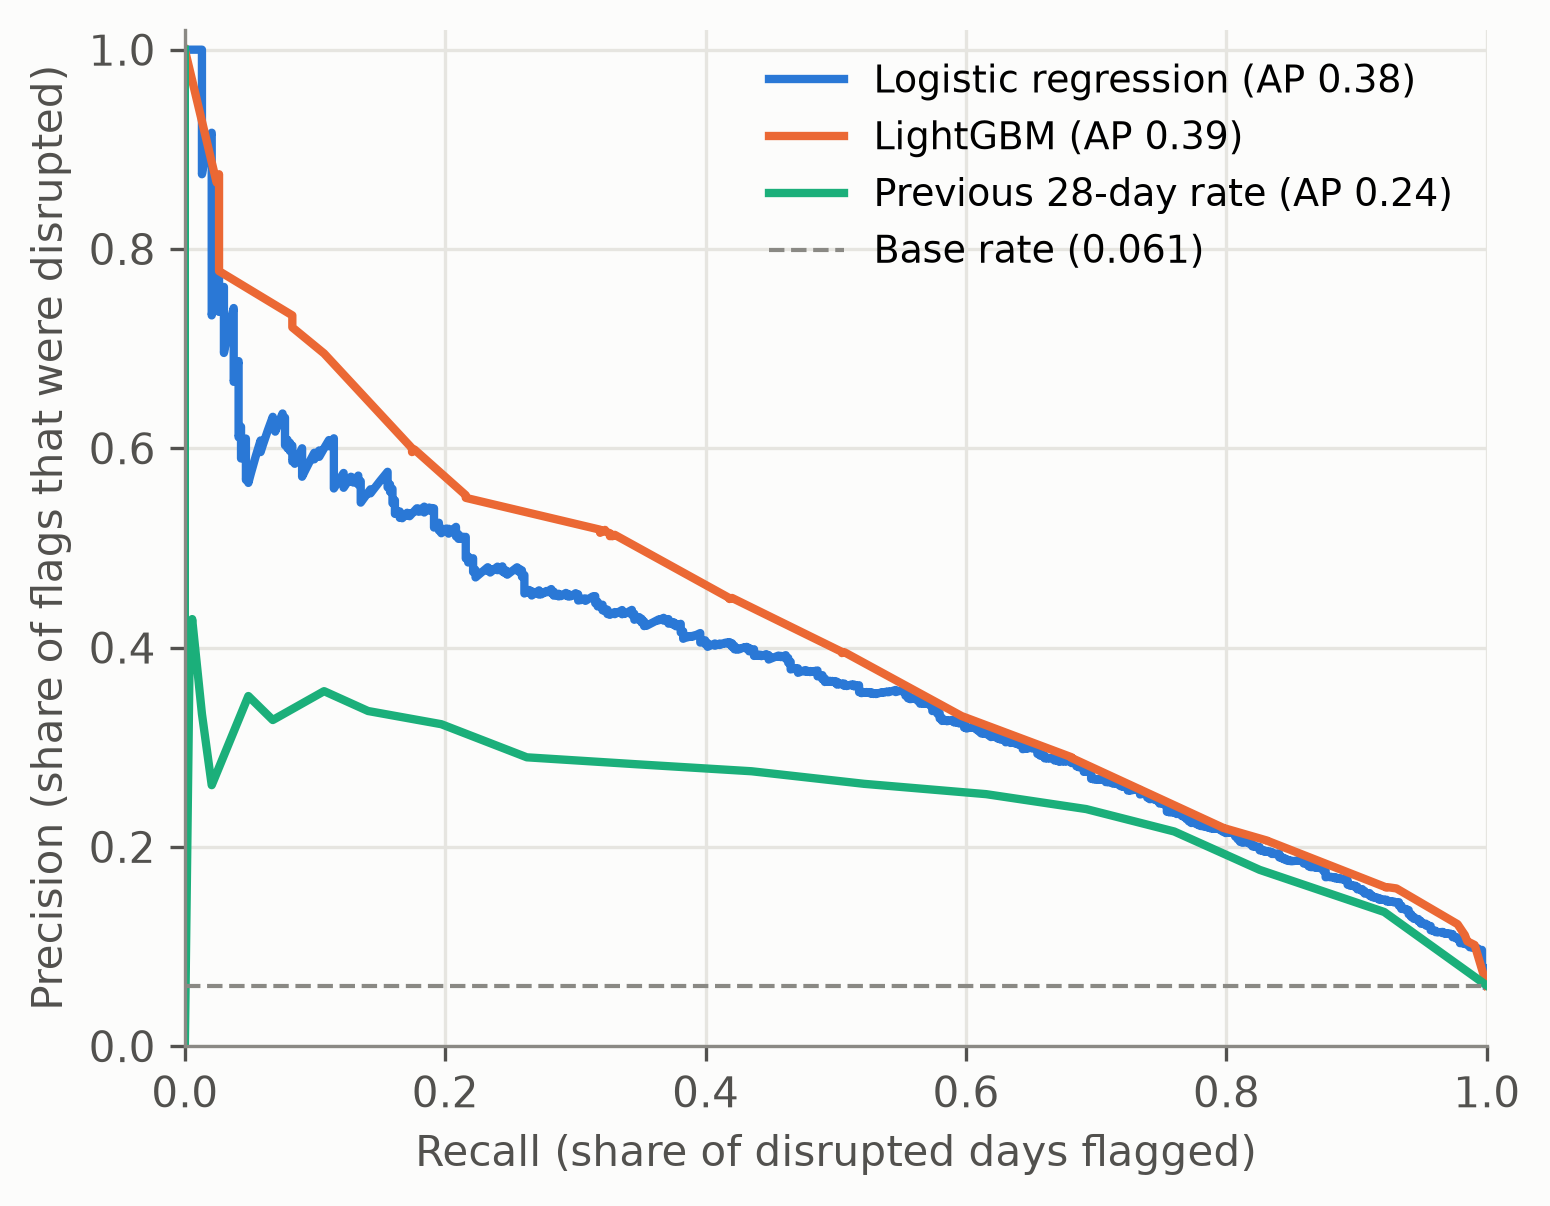
\includegraphics[width=0.5\linewidth]{panel1_precision_recall_2024_2025.png}\\[0.3em]
{\footnotesize \textbf{Fig.~1A} Precision--recall curves on the 2024--2025 test years for logistic regression, LightGBM and the previous 28-day disruption rate; dashed line: base rate.}
\end{center}

%% Description: Background & Results
\paragraph{Background}
When an airport cannot accept all planned arrivals, EUROCONTROL's Network Manager holds flights at their departure airports. The resulting air traffic flow management (ATFM) delay is published per airport and day, with its cause [1, 2]. Weather is the largest recorded cause at German airports: 67\% of all ATFM arrival delay minutes at the 12 airports studied here, 2014--2025. We asked whether public traffic and weather data are enough to anticipate which airport-days will be disrupted, defined as days on which at least 2\% of arrivals receive more than 15 minutes of ATFM delay (6.2\% of airport-days; 19.4\% at Frankfurt).

\paragraph{Results}
We joined daily EUROCONTROL arrival delays [Data 1] with hourly observations from the DWD station at each airport [Data 2] into 52,596 airport-days (\href{\repo/blob/main/figures/panel5_data_pipeline.png}{Fig.~1E}; all processing steps in [Protocol 1]). Models used 37 predictors: calendar, traffic and delay history from earlier days only, and same-day observed weather as a stand-in for a perfect forecast. They were trained on 2014--2021, tuned on 2022, calibrated on 2023 and scored once on 2024--2025 (8,771 airport-days, 533 disrupted).

LightGBM [4] reached an average precision (AP) of 0.39 and a ROC-AUC of 0.90; logistic regression [3] reached 0.38 and 0.89 (Fig.~1A). At an alert threshold of 0.20 chosen on 2023, LightGBM flagged 682 days with a precision of 0.39 and a recall of 0.50. The gain over recent history was largest at Frankfurt (AP 0.63 vs 0.30) and smallest at Stuttgart, where both models caught only 3 of 52 disrupted days (\href{\repo/blob/main/figures/panel2_average_precision_by_airport.png}{Fig.~1B}).

The descriptive analysis points to weather and traffic. Thunderstorm days were 3.9 to 5.5 times as likely to be disrupted as other days at Frankfurt, Munich and Stuttgart (\href{\repo/blob/main/figures/panel3_weather_risk_ratio_by_airport.png}{Fig.~1C}). Disruption rose with traffic and with the number of adverse weather conditions, reaching 25.5\% on days with two conditions and 100--120\% of the airport's median traffic (\href{\repo/blob/main/figures/panel4_disruption_by_traffic_and_weather.png}{Fig.~1D}). Predicting delay minutes per arrival was harder: LightGBM barely beat predicting zero (MAE 0.200 vs 0.207). Because observed weather replaces a forecast, all scores are an upper bound for day-ahead use.


{\footnotesize
\textbf{Further panels:}
\href{\repo/blob/main/figures/panel2_average_precision_by_airport.png}{1B Average precision by airport (airports with at least 20 disrupted test days)};
\href{\repo/blob/main/figures/panel3_weather_risk_ratio_by_airport.png}{1C Disruption risk ratio by weather condition and airport, 2014--2025 (grey: fewer than 10 disrupted days, n = disrupted days)};
\href{\repo/blob/main/figures/panel4_disruption_by_traffic_and_weather.png}{1D Disruption rate by traffic relative to the airport's median in the same year and number of adverse weather conditions (grey: fewer than 50 days)};
\href{\repo/blob/main/figures/panel5_data_pipeline.png}{1E From raw sources to the airport-day table, BI notebooks and models}.
}

%% References
\paragraph{References}
\begin{enumerate}[label={[\arabic*]}]
\item EUROCONTROL Performance Review Unit. ATFM delay definition. \url{https://ansperformance.eu/definition/atfm-delay/}
\item EUROCONTROL Performance Review Unit. Airport arrival ATFM delays. \url{https://ansperformance.eu/capacity/atfm_apt}
\item Pedregosa, F.\ et al.\ (2011). Scikit-learn: Machine Learning in Python. \textit{Journal of Machine Learning Research} 12, 2825--2830. \url{https://jmlr.org/papers/v12/pedregosa11a.html}
\item Ke, G.\ et al.\ (2017). LightGBM: A Highly Efficient Gradient Boosting Decision Tree. \textit{Advances in Neural Information Processing Systems} 30. \url{https://proceedings.neurips.cc/paper/2017/hash/6449f44a102fde848669bdd9eb6b76fa-Abstract.html}
\end{enumerate}

%% Code
\paragraph{Code}
\begin{enumerate}[label={[\arabic*]}]
\item Project repository: data pipeline, BI and model notebooks, figure script. \url{\repo}
\end{enumerate}

%% Data
\paragraph{Data}
\begin{enumerate}[label={[\arabic*]}]
\item EUROCONTROL. Daily airport arrival ATFM delay files \texttt{apt\_dly\_YYYY.csv.bz2}, 2014--2025. \url{https://www.eurocontrol.int/performance/data/download/csv/apt_dly_2025.csv.bz2} (one file per year)
\item Deutscher Wetterdienst, Climate Data Center. Hourly station observations (CC BY 4.0). \url{https://opendata.dwd.de/climate_environment/CDC/observations_germany/climate/hourly/}
\item Processed dataset (52,596 airport-days, 79 columns) with feature contract and quality report. \url{\repo/tree/main/data/processed}
\end{enumerate}

%% Protocols
\paragraph{Protocols}
\begin{enumerate}[label={[\arabic*]}]
\item Data sources and processing: download, cleaning, hourly-to-daily aggregation, targets and features. \url{\repo/blob/main/docs/DATA.md}
\item Model training and evaluation protocol (time-based split, tuning, calibration, single test evaluation). \url{\repo/tree/main/notebooks}
\end{enumerate}

\end{document}
